\chapter{Design methodology} \label{ch:designmet}
\todo{læs om system design methodologies i gajski's \textbf{Embedded Systems Design - Modeling, Synthesis and Verification} og beskriv Platform Methodology}
In \cite{gajski2009} the Gajski-Kuhn Y-chart is described and it is illustrated on figure \ref{fig:ychart_std}. This chart can help describe a way to design a system. It moves between the three domains: Behaviour, Structure and Physical.
\begin{figure}[ht]
  \centering
  \begin{subfigure}[t]{0.475\textwidth}
    \centering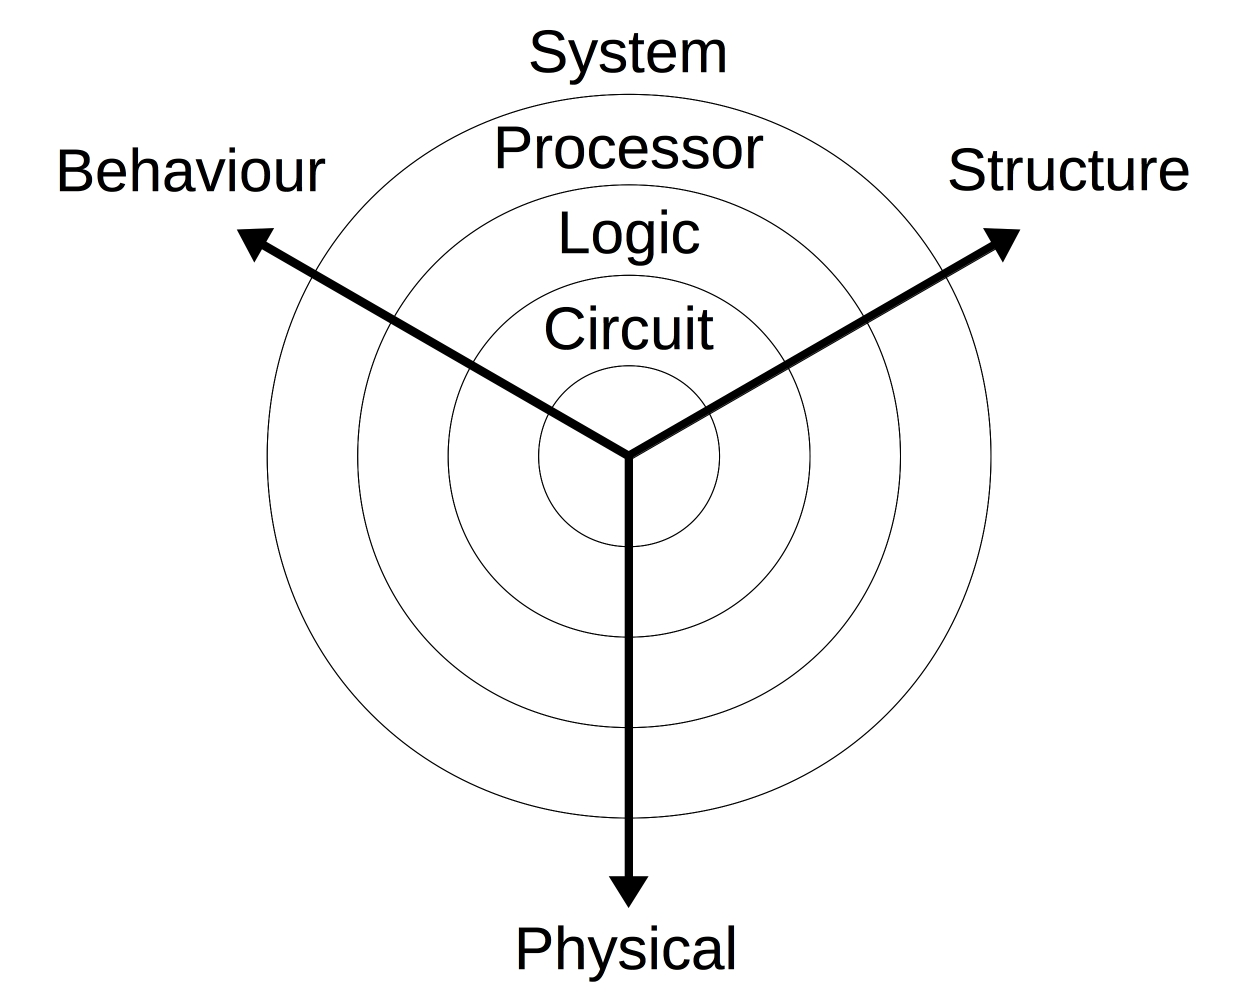
\includegraphics[width=\textwidth]{figures/ychart-std.jpg}
    \caption{Illustration of the standard Gajski-Kuhn Y-chart \cite{gajski2009}\label{fig:ychart_std}}
  \end{subfigure}\hspace{0.25cm}
  \begin{subfigure}[t]{0.475\textwidth}
    \centering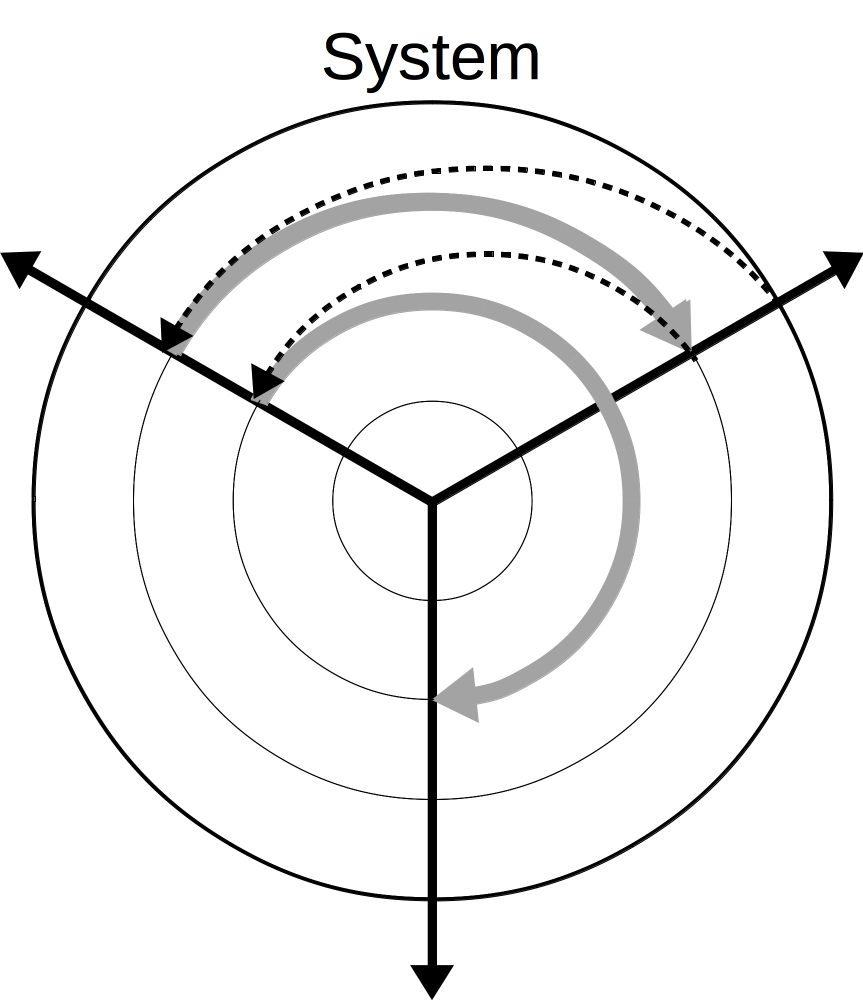
\includegraphics[width=\textwidth]{figures/ychart-fpga.jpg}
    \caption{Illustration of the Gajski-Kuhn Y-chart showing the FPGA methodology \cite{gajski2009}  \label{fig:ychart_fpga}}
  \end{subfigure}\hspace{0.5cm}
  \caption{Illustrations of Gajski-Kuhn Y-chart\label{fig:ychartall}}
\end{figure}

\color{gray}
\section*{noter til mig selv}
% --------------------------- udkommentere senere ------
processor synthesis:\\
side 32 i gajski pdf \\
(a) allocation of components and connections \\
(b) cycle-accurate scheduling\\
(c) Binding of variables, operations and transfers\\
(d) Synthesis of controller\\
(e) Model refinement\\
(a-c) kan udføres sammen eller i hvilken som helst rækkefølge men de er afhængige af hinanden. Hvis de udføres samtidigt bliver synthesen kompleks og utilregnlig. en strategi er at udføre det i følgende rækkefølge: a c b\\
Alle trinene ovenover kan udføres automatisk eller manuelt. Hvis det hele bliver udført automatisk kaldes det processor-level synthesis eller high-level synthesis (HLS).  Hvis a-d blvier udført manuelt og e automatisk kaldes det model refinement.\\
\\
System-level behavioral model / system synthesis: side 35\\
(a) Profiling and estimation. \\
(b) Component and connection allocation\\
(c) Process and channel binding\\
(d) Process scheduling\\
(e) IF component insertion\\
(f) Model refinement\\
\\
1.3 System Design methodology: side 39 \\
model algebra side 42\\
algebra:<objects, operations>\\
$a*(b+c) = a*b+a*c$\\
dette gør det muligt for system designere at optimere designet vha. arithmetic algebra regler. Udtrykket til venstre for = kræver en multiplier og en adder hvorimod udtrykket på højre side kræver 2 multipliers og en adder.\\
modelalgebra : <objects, compositions>\\
\\
1.4 System-level models: side 44\\
applications designers, system designers og implementations designers.\\
\\
2 system design methodologies side 56\\
Dette kapitel beskriver forskellige system design methodologies.\\
Bottom-up: start i bunden (circuit level) kør fra behavior til physical og lav et library. brug dette library til næste level.\\
Top-down: Start i øverste level (system level) kør fra behavior over til structure. gå et level ned og gentag. ved nederste level gå fra behavior til physical.\\
Platform methodology: side 61\\
FPGA methodology: side 64\\
er based på FPGA substrat som består af multitude af 4-bits ROM celler (Look-up Tables (LUTs)) og disse LUTs kan implementere enhver 4-variable boolsk funktion. I denne design methodologi vil hver RTL kompement in biblioteket være opbygget af disse 4-variable funktioner. Og derefter bliver processor delene synthesizeret af disse RTL componenter.\\
sagt på en anden måde: denne methodologi bruger en top-down approach på både system og processor levels hvor standard og custom Processing Elements og Communication Elements er opbygget af LUTs. Et system design starter ved at man mapper en applikation ned på en given platform og derefter syntheser brugerdefineret kompenenter ned til RTL komponenter som er defineret in form af LUTs. Standard processor komponenter i processor biblioteket er allerede defineret i form af LUTs. Når alle vores komponenter er defineret vha LUTs så simplificere vi designet ned til LUTs og BRAM og derefter kan vi udføre placering og routing med værktøjer FPGA producentet har udviklet.\\
Denne form for top-down metode har de samme svagheder som andre top-down metoder som er at det kan være svært at optimere hele designet ved at simplificere designet ned til basiske LUT celler. Derudover ved udvikler heller ikke om hvordan FPGA producentens værktøj placerere og forbinder LUTs og BRAMs.\\


\color{black}






